\documentclass[1p]{elsarticle_modified}
%\bibliographystyle{elsarticle-num}

%\usepackage[colorlinks]{hyperref}
%\usepackage{abbrmath_seonhwa} %\Abb, \Ascr, \Acal ,\Abf, \Afrak
\usepackage{amsfonts}
\usepackage{amssymb}
\usepackage{amsmath}
\usepackage{amsthm}
\usepackage{scalefnt}
\usepackage{amsbsy}
\usepackage{kotex}
\usepackage{caption}
\usepackage{subfig}
\usepackage{color}
\usepackage{graphicx}
\usepackage{xcolor} %% white, black, red, green, blue, cyan, magenta, yellow
\usepackage{float}
\usepackage{setspace}
\usepackage{hyperref}

\usepackage{tikz}
\usetikzlibrary{arrows}

\usepackage{multirow}
\usepackage{array} % fixed length table
\usepackage{hhline}

%%%%%%%%%%%%%%%%%%%%%
\makeatletter
\renewcommand*\env@matrix[1][\arraystretch]{%
	\edef\arraystretch{#1}%
	\hskip -\arraycolsep
	\let\@ifnextchar\new@ifnextchar
	\array{*\c@MaxMatrixCols c}}
\makeatother %https://tex.stackexchange.com/questions/14071/how-can-i-increase-the-line-spacing-in-a-matrix
%%%%%%%%%%%%%%%

\usepackage[normalem]{ulem}

\newcommand{\msout}[1]{\ifmmode\text{\sout{\ensuremath{#1}}}\else\sout{#1}\fi}
%SOURCE: \msout is \stkout macro in https://tex.stackexchange.com/questions/20609/strikeout-in-math-mode

\newcommand{\cancel}[1]{
	\ifmmode
	{\color{red}\msout{#1}}
	\else
	{\color{red}\sout{#1}}
	\fi
}

\newcommand{\add}[1]{
	{\color{blue}\uwave{#1}}
}

\newcommand{\replace}[2]{
	\ifmmode
	{\color{red}\msout{#1}}{\color{blue}\uwave{#2}}
	\else
	{\color{red}\sout{#1}}{\color{blue}\uwave{#2}}
	\fi
}

\newcommand{\Sol}{\mathcal{S}} %segment
\newcommand{\D}{D} %diagram
\newcommand{\A}{\mathcal{A}} %arc


%%%%%%%%%%%%%%%%%%%%%%%%%%%%%5 test

\def\sl{\operatorname{\textup{SL}}(2,\Cbb)}
\def\psl{\operatorname{\textup{PSL}}(2,\Cbb)}
\def\quan{\mkern 1mu \triangleright \mkern 1mu}

\theoremstyle{definition}
\newtheorem{thm}{Theorem}[section]
\newtheorem{prop}[thm]{Proposition}
\newtheorem{lem}[thm]{Lemma}
\newtheorem{ques}[thm]{Question}
\newtheorem{cor}[thm]{Corollary}
\newtheorem{defn}[thm]{Definition}
\newtheorem{exam}[thm]{Example}
\newtheorem{rmk}[thm]{Remark}
\newtheorem{alg}[thm]{Algorithm}

\newcommand{\I}{\sqrt{-1}}
\begin{document}

%\begin{frontmatter}
%
%\title{Boundary parabolic representations of knots up to 8 crossings}
%
%%% Group authors per affiliation:
%\author{Yunhi Cho} 
%\address{Department of Mathematics, University of Seoul, Seoul, Korea}
%\ead{yhcho@uos.ac.kr}
%
%
%\author{Seonhwa Kim} %\fnref{s_kim}}
%\address{Center for Geometry and Physics, Institute for Basic Science, Pohang, 37673, Korea}
%\ead{ryeona17@ibs.re.kr}
%
%\author{Hyuk Kim}
%\address{Department of Mathematical Sciences, Seoul National University, Seoul 08826, Korea}
%\ead{hyukkim@snu.ac.kr}
%
%\author{Seokbeom Yoon}
%\address{Department of Mathematical Sciences, Seoul National University, Seoul, 08826,  Korea}
%\ead{sbyoon15@snu.ac.kr}
%
%\begin{abstract}
%We find all boundary parabolic representation of knots up to 8 crossings.
%
%\end{abstract}
%\begin{keyword}
%    \MSC[2010] 57M25 
%\end{keyword}
%
%\end{frontmatter}

%\linenumbers
%\tableofcontents
%
\newcommand\colored[1]{\textcolor{white}{\rule[-0.35ex]{0.8em}{1.4ex}}\kern-0.8em\color{red} #1}%
%\newcommand\colored[1]{\textcolor{white}{ #1}\kern-2.17ex	\textcolor{white}{ #1}\kern-1.81ex	\textcolor{white}{ #1}\kern-2.15ex\color{red}#1	}

{\Large $\underline{12a_{0654}~(K12a_{0654})}$}

\setlength{\tabcolsep}{10pt}
\renewcommand{\arraystretch}{1.6}
\vspace{1cm}\begin{tabular}{m{100pt}>{\centering\arraybackslash}m{274pt}}
\multirow{5}{120pt}{
	\centering
	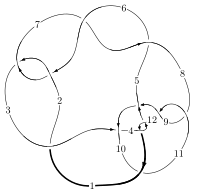
\includegraphics[width=112pt]{../../../GIT/diagram.site/Diagrams/png/1455_12a_0654.png}\\
\ \ \ A knot diagram\footnotemark}&
\allowdisplaybreaks
\textbf{Linearized knot diagam} \\
\cline{2-2}
 &
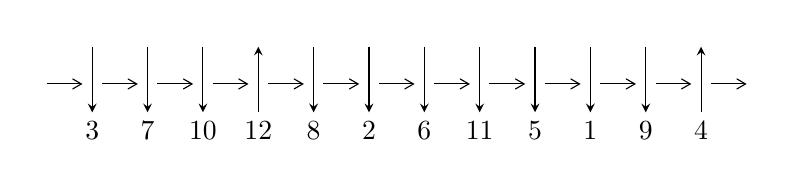
\begin{tikzpicture}[x=20pt, y=17pt]
	% nodes
	\node (C0) at (0, 0) {};
	\node (C1) at (1, 0) {};
	\node (C1U) at (1, +1) {};
	\node (C1D) at (1, -1) {3};

	\node (C2) at (2, 0) {};
	\node (C2U) at (2, +1) {};
	\node (C2D) at (2, -1) {7};

	\node (C3) at (3, 0) {};
	\node (C3U) at (3, +1) {};
	\node (C3D) at (3, -1) {10};

	\node (C4) at (4, 0) {};
	\node (C4U) at (4, +1) {};
	\node (C4D) at (4, -1) {12};

	\node (C5) at (5, 0) {};
	\node (C5U) at (5, +1) {};
	\node (C5D) at (5, -1) {8};

	\node (C6) at (6, 0) {};
	\node (C6U) at (6, +1) {};
	\node (C6D) at (6, -1) {2};

	\node (C7) at (7, 0) {};
	\node (C7U) at (7, +1) {};
	\node (C7D) at (7, -1) {6};

	\node (C8) at (8, 0) {};
	\node (C8U) at (8, +1) {};
	\node (C8D) at (8, -1) {11};

	\node (C9) at (9, 0) {};
	\node (C9U) at (9, +1) {};
	\node (C9D) at (9, -1) {5};

	\node (C10) at (10, 0) {};
	\node (C10U) at (10, +1) {};
	\node (C10D) at (10, -1) {1};

	\node (C11) at (11, 0) {};
	\node (C11U) at (11, +1) {};
	\node (C11D) at (11, -1) {9};

	\node (C12) at (12, 0) {};
	\node (C12U) at (12, +1) {};
	\node (C12D) at (12, -1) {4};
	\node (C13) at (13, 0) {};

	% arrows
	\draw[->,>={angle 60}]
	(C0) edge (C1) (C1) edge (C2) (C2) edge (C3) (C3) edge (C4) (C4) edge (C5) (C5) edge (C6) (C6) edge (C7) (C7) edge (C8) (C8) edge (C9) (C9) edge (C10) (C10) edge (C11) (C11) edge (C12) (C12) edge (C13) ;	\draw[->,>=stealth]
	(C1U) edge (C1D) (C2U) edge (C2D) (C3U) edge (C3D) (C4D) edge (C4U) (C5U) edge (C5D) (C6U) edge (C6D) (C7U) edge (C7D) (C8U) edge (C8D) (C9U) edge (C9D) (C10U) edge (C10D) (C11U) edge (C11D) (C12D) edge (C12U) ;
	\end{tikzpicture} \\
\hhline{~~} \\& 
\textbf{Solving Sequence} \\ \cline{2-2} 
 &
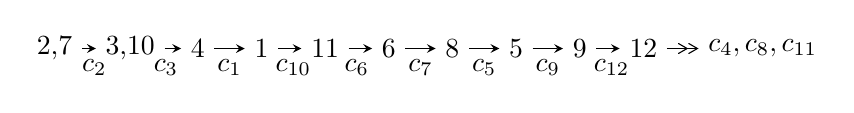
\begin{tikzpicture}[x=23pt, y=7pt]
	% node
	\node (A0) at (-1/8, 0) {2,7};
	\node (A1) at (17/16, 0) {3,10};
	\node (A2) at (17/8, 0) {4};
	\node (A3) at (25/8, 0) {1};
	\node (A4) at (33/8, 0) {11};
	\node (A5) at (41/8, 0) {6};
	\node (A6) at (49/8, 0) {8};
	\node (A7) at (57/8, 0) {5};
	\node (A8) at (65/8, 0) {9};
	\node (A9) at (73/8, 0) {12};
	\node (C1) at (1/2, -1) {$c_{2}$};
	\node (C2) at (13/8, -1) {$c_{3}$};
	\node (C3) at (21/8, -1) {$c_{1}$};
	\node (C4) at (29/8, -1) {$c_{10}$};
	\node (C5) at (37/8, -1) {$c_{6}$};
	\node (C6) at (45/8, -1) {$c_{7}$};
	\node (C7) at (53/8, -1) {$c_{5}$};
	\node (C8) at (61/8, -1) {$c_{9}$};
	\node (C9) at (69/8, -1) {$c_{12}$};
	\node (A10) at (11, 0) {$c_{4},c_{8},c_{11}$};

	% edge
	\draw[->,>=stealth]	
	(A0) edge (A1) (A1) edge (A2) (A2) edge (A3) (A3) edge (A4) (A4) edge (A5) (A5) edge (A6) (A6) edge (A7) (A7) edge (A8) (A8) edge (A9) ;
	\draw[->>,>={angle 60}]	
	(A9) edge (A10);
\end{tikzpicture} \\ 

\end{tabular} \\

\footnotetext{
The image of knot diagram is generated by the software ``\textbf{Draw programme}" developed by Andrew Bartholomew(\url{http://www.layer8.co.uk/maths/draw/index.htm\#Running-draw}), where we modified some parts for our purpose(\url{https://github.com/CATsTAILs/LinksPainter}).
}\phantom \\ \newline 
\centering \textbf{Ideals for irreducible components\footnotemark of $X_{\text{par}}$} 
 
\begin{align*}
I^u_{1}&=\langle 
1.44776\times10^{45} u^{82}+1.88228\times10^{45} u^{81}+\cdots+4.67106\times10^{45} b-4.92257\times10^{45},\\
\phantom{I^u_{1}}&\phantom{= \langle  }4.56361\times10^{45} u^{82}+3.89164\times10^{45} u^{81}+\cdots+4.67106\times10^{45} a+4.38504\times10^{45},\;u^{83}+2 u^{82}+\cdots+2 u-1\rangle \\
I^u_{2}&=\langle 
2 b+1,\;2 a+1,\;u-1\rangle \\
\\
\end{align*}
\raggedright * 2 irreducible components of $\dim_{\mathbb{C}}=0$, with total 84 representations.\\
\footnotetext{All coefficients of polynomials are rational numbers. But the coefficients are sometimes approximated in decimal forms when there is not enough margin.}
\newpage
\renewcommand{\arraystretch}{1}
\centering \section*{I. $I^u_{1}= \langle 1.45\times10^{45} u^{82}+1.88\times10^{45} u^{81}+\cdots+4.67\times10^{45} b-4.92\times10^{45},\;4.56\times10^{45} u^{82}+3.89\times10^{45} u^{81}+\cdots+4.67\times10^{45} a+4.39\times10^{45},\;u^{83}+2 u^{82}+\cdots+2 u-1 \rangle$}
\flushleft \textbf{(i) Arc colorings}\\
\begin{tabular}{m{7pt} m{180pt} m{7pt} m{180pt} }
\flushright $a_{2}=$&$\begin{pmatrix}1\\0\end{pmatrix}$ \\
\flushright $a_{7}=$&$\begin{pmatrix}0\\u\end{pmatrix}$ \\
\flushright $a_{3}=$&$\begin{pmatrix}1\\u^2\end{pmatrix}$ \\
\flushright $a_{10}=$&$\begin{pmatrix}-0.976996 u^{82}-0.833138 u^{81}+\cdots-1.67953 u-0.938767\\-0.309942 u^{82}-0.402967 u^{81}+\cdots-0.857176 u+1.05384\end{pmatrix}$ \\
\flushright $a_{4}=$&$\begin{pmatrix}0.490538 u^{82}+0.276265 u^{81}+\cdots+1.57387 u-1.06664\\0.136027 u^{82}+0.165051 u^{81}+\cdots+0.892769 u-0.223335\end{pmatrix}$ \\
\flushright $a_{1}=$&$\begin{pmatrix}- u^2+1\\- u^4\end{pmatrix}$ \\
\flushright $a_{11}=$&$\begin{pmatrix}-1.04749 u^{82}-0.897950 u^{81}+\cdots-1.23217 u-1.87684\\-1.54527 u^{82}-1.66408 u^{81}+\cdots-1.87786 u+1.38750\end{pmatrix}$ \\
\flushright $a_{6}=$&$\begin{pmatrix}u\\u\end{pmatrix}$ \\
\flushright $a_{8}=$&$\begin{pmatrix}- u^3\\- u^3+u\end{pmatrix}$ \\
\flushright $a_{5}=$&$\begin{pmatrix}u^5+u\\u^5- u^3+u\end{pmatrix}$ \\
\flushright $a_{9}=$&$\begin{pmatrix}-0.921584 u^{82}-0.763915 u^{81}+\cdots+0.687349 u-1.85196\\-1.37611 u^{82}-1.44172 u^{81}+\cdots-0.552013 u+1.27476\end{pmatrix}$ \\
\flushright $a_{12}=$&$\begin{pmatrix}0.374473 u^{82}+0.269946 u^{81}+\cdots+3.53516 u+0.0915879\\0.597808 u^{82}+0.580589 u^{81}+\cdots+1.55233 u-0.354511\end{pmatrix}$\\&\end{tabular}
\flushleft \textbf{(ii) Obstruction class $= -1$}\\~\\
\flushleft \textbf{(iii) Cusp Shapes $= 1.68031 u^{82}-1.52488 u^{81}+\cdots-2.18584 u-10.4378$}\\~\\
\newpage\renewcommand{\arraystretch}{1}
\flushleft \textbf{(iv) u-Polynomials at the component}\newline \\
\begin{tabular}{m{50pt}|m{274pt}}
Crossings & \hspace{64pt}u-Polynomials at each crossing \\
\hline $$\begin{aligned}c_{1},c_{5},c_{7}\end{aligned}$$&$\begin{aligned}
&u^{83}+20 u^{82}+\cdots+12 u+1
\end{aligned}$\\
\hline $$\begin{aligned}c_{2},c_{6}\end{aligned}$$&$\begin{aligned}
&u^{83}-2 u^{82}+\cdots+2 u+1
\end{aligned}$\\
\hline $$\begin{aligned}c_{3}\end{aligned}$$&$\begin{aligned}
&u^{83}+u^{82}+\cdots-62 u+8
\end{aligned}$\\
\hline $$\begin{aligned}c_{4},c_{12}\end{aligned}$$&$\begin{aligned}
&u^{83}+4 u^{82}+\cdots+4 u+1
\end{aligned}$\\
\hline $$\begin{aligned}c_{8},c_{11}\end{aligned}$$&$\begin{aligned}
&u^{83}-2 u^{82}+\cdots-35 u+4
\end{aligned}$\\
\hline $$\begin{aligned}c_{9}\end{aligned}$$&$\begin{aligned}
&2(2 u^{83}+13 u^{82}+\cdots-65101 u+15173)
\end{aligned}$\\
\hline $$\begin{aligned}c_{10}\end{aligned}$$&$\begin{aligned}
&2(2 u^{83}+35 u^{82}+\cdots+62 u-4)
\end{aligned}$\\
\hline
\end{tabular}\\~\\
\newpage\renewcommand{\arraystretch}{1}
\flushleft \textbf{(v) Riley Polynomials at the component}\newline \\
\begin{tabular}{m{50pt}|m{274pt}}
Crossings & \hspace{64pt}Riley Polynomials at each crossing \\
\hline $$\begin{aligned}c_{1},c_{5},c_{7}\end{aligned}$$&$\begin{aligned}
&y^{83}+88 y^{82}+\cdots-40 y-1
\end{aligned}$\\
\hline $$\begin{aligned}c_{2},c_{6}\end{aligned}$$&$\begin{aligned}
&y^{83}-20 y^{82}+\cdots+12 y-1
\end{aligned}$\\
\hline $$\begin{aligned}c_{3}\end{aligned}$$&$\begin{aligned}
&y^{83}+9 y^{82}+\cdots-2956 y-64
\end{aligned}$\\
\hline $$\begin{aligned}c_{4},c_{12}\end{aligned}$$&$\begin{aligned}
&y^{83}+60 y^{82}+\cdots+12 y-1
\end{aligned}$\\
\hline $$\begin{aligned}c_{8},c_{11}\end{aligned}$$&$\begin{aligned}
&y^{83}-52 y^{82}+\cdots+1569 y-16
\end{aligned}$\\
\hline $$\begin{aligned}c_{9}\end{aligned}$$&$\begin{aligned}
&4(4 y^{83}+507 y^{82}+\cdots+8.37318\times10^{9} y-2.30220\times10^{8})
\end{aligned}$\\
\hline $$\begin{aligned}c_{10}\end{aligned}$$&$\begin{aligned}
&4(4 y^{83}-677 y^{82}+\cdots+156 y-16)
\end{aligned}$\\
\hline
\end{tabular}\\~\\
\newpage\flushleft \textbf{(vi) Complex Volumes and Cusp Shapes}
$$\begin{array}{c|c|c}  
\text{Solutions to }I^u_{1}& \I (\text{vol} + \sqrt{-1}CS) & \text{Cusp shape}\\
 \hline 
\begin{aligned}
u &= \phantom{-}0.903364 + 0.424677 I \\
a &= \phantom{-}1.53894 - 1.55609 I \\
b &= \phantom{-}0.888909 - 0.865193 I\end{aligned}
 & -1.93320 - 6.97812 I & \phantom{-0.000000 } 0 \\ \hline\begin{aligned}
u &= \phantom{-}0.903364 - 0.424677 I \\
a &= \phantom{-}1.53894 + 1.55609 I \\
b &= \phantom{-}0.888909 + 0.865193 I\end{aligned}
 & -1.93320 + 6.97812 I & \phantom{-0.000000 } 0 \\ \hline\begin{aligned}
u &= -0.867473 + 0.468864 I \\
a &= -1.15941 - 0.99435 I \\
b &= -0.875451 - 0.381159 I\end{aligned}
 & \phantom{-}1.31046 + 3.33552 I & \phantom{-0.000000 } 0 \\ \hline\begin{aligned}
u &= -0.867473 - 0.468864 I \\
a &= -1.15941 + 0.99435 I \\
b &= -0.875451 + 0.381159 I\end{aligned}
 & \phantom{-}1.31046 - 3.33552 I & \phantom{-0.000000 } 0 \\ \hline\begin{aligned}
u &= -1.042220 + 0.035267 I \\
a &= -0.793950 - 0.624964 I \\
b &= \phantom{-}0.087591 + 0.119886 I\end{aligned}
 & -8.94189 - 6.52162 I & \phantom{-0.000000 } 0 \\ \hline\begin{aligned}
u &= -1.042220 - 0.035267 I \\
a &= -0.793950 + 0.624964 I \\
b &= \phantom{-}0.087591 - 0.119886 I\end{aligned}
 & -8.94189 + 6.52162 I & \phantom{-0.000000 } 0 \\ \hline\begin{aligned}
u &= -0.878924 + 0.323578 I \\
a &= \phantom{-}0.58100 - 1.29209 I \\
b &= \phantom{-}1.053830 - 0.003673 I\end{aligned}
 & -6.40049 + 4.26517 I & -17.4265 - 8.0576 I \\ \hline\begin{aligned}
u &= -0.878924 - 0.323578 I \\
a &= \phantom{-}0.58100 + 1.29209 I \\
b &= \phantom{-}1.053830 + 0.003673 I\end{aligned}
 & -6.40049 - 4.26517 I & -17.4265 + 8.0576 I \\ \hline\begin{aligned}
u &= \phantom{-}0.813017 + 0.384092 I \\
a &= -0.00859 - 1.76199 I \\
b &= \phantom{-}0.676319 - 0.764949 I\end{aligned}
 & -2.07969 - 1.17143 I & -10.66001 + 4.16977 I \\ \hline\begin{aligned}
u &= \phantom{-}0.813017 - 0.384092 I \\
a &= -0.00859 + 1.76199 I \\
b &= \phantom{-}0.676319 + 0.764949 I\end{aligned}
 & -2.07969 + 1.17143 I & -10.66001 - 4.16977 I\\
 \hline 
 \end{array}$$\newpage$$\begin{array}{c|c|c}  
\text{Solutions to }I^u_{1}& \I (\text{vol} + \sqrt{-1}CS) & \text{Cusp shape}\\
 \hline 
\begin{aligned}
u &= \phantom{-}0.420879 + 0.791590 I \\
a &= -0.598628 - 0.823093 I \\
b &= \phantom{-}0.147354 - 0.727487 I\end{aligned}
 & -3.58940 - 5.15177 I & -8.49512 + 7.35556 I \\ \hline\begin{aligned}
u &= \phantom{-}0.420879 - 0.791590 I \\
a &= -0.598628 + 0.823093 I \\
b &= \phantom{-}0.147354 + 0.727487 I\end{aligned}
 & -3.58940 + 5.15177 I & -8.49512 - 7.35556 I \\ \hline\begin{aligned}
u &= \phantom{-}1.013160 + 0.441729 I \\
a &= -1.39941 + 1.30714 I \\
b &= -1.24596 + 0.86067 I\end{aligned}
 & -6.5398 - 12.7131 I & \phantom{-0.000000 } 0 \\ \hline\begin{aligned}
u &= \phantom{-}1.013160 - 0.441729 I \\
a &= -1.39941 - 1.30714 I \\
b &= -1.24596 - 0.86067 I\end{aligned}
 & -6.5398 + 12.7131 I & \phantom{-0.000000 } 0 \\ \hline\begin{aligned}
u &= \phantom{-}0.823581 + 0.346061 I \\
a &= \phantom{-}0.938555 - 0.307109 I \\
b &= \phantom{-}0.017949 + 0.810468 I\end{aligned}
 & -2.23914 - 2.76864 I & -10.20780 + 5.54130 I \\ \hline\begin{aligned}
u &= \phantom{-}0.823581 - 0.346061 I \\
a &= \phantom{-}0.938555 + 0.307109 I \\
b &= \phantom{-}0.017949 - 0.810468 I\end{aligned}
 & -2.23914 + 2.76864 I & -10.20780 - 5.54130 I \\ \hline\begin{aligned}
u &= -1.027830 + 0.414105 I \\
a &= \phantom{-}1.072000 + 0.556379 I \\
b &= \phantom{-}0.807846 + 0.347687 I\end{aligned}
 & -1.47818 + 7.11634 I & \phantom{-0.000000 } 0 \\ \hline\begin{aligned}
u &= -1.027830 - 0.414105 I \\
a &= \phantom{-}1.072000 - 0.556379 I \\
b &= \phantom{-}0.807846 - 0.347687 I\end{aligned}
 & -1.47818 - 7.11634 I & \phantom{-0.000000 } 0 \\ \hline\begin{aligned}
u &= \phantom{-}0.849599 + 0.221125 I \\
a &= -2.26382 + 0.89058 I \\
b &= -1.08261 + 1.27189 I\end{aligned}
 & -6.96103 - 0.26061 I & -19.4591 + 2.1398 I \\ \hline\begin{aligned}
u &= \phantom{-}0.849599 - 0.221125 I \\
a &= -2.26382 - 0.89058 I \\
b &= -1.08261 - 1.27189 I\end{aligned}
 & -6.96103 + 0.26061 I & -19.4591 - 2.1398 I\\
 \hline 
 \end{array}$$\newpage$$\begin{array}{c|c|c}  
\text{Solutions to }I^u_{1}& \I (\text{vol} + \sqrt{-1}CS) & \text{Cusp shape}\\
 \hline 
\begin{aligned}
u &= \phantom{-}1.119060 + 0.149420 I \\
a &= \phantom{-}0.014858 - 0.335944 I \\
b &= -0.0823966 - 0.0099121 I\end{aligned}
 & -3.26358 + 0.42527 I & \phantom{-0.000000 } 0 \\ \hline\begin{aligned}
u &= \phantom{-}1.119060 - 0.149420 I \\
a &= \phantom{-}0.014858 + 0.335944 I \\
b &= -0.0823966 + 0.0099121 I\end{aligned}
 & -3.26358 - 0.42527 I & \phantom{-0.000000 } 0 \\ \hline\begin{aligned}
u &= \phantom{-}1.040690 + 0.521910 I \\
a &= \phantom{-}0.526785 + 0.646610 I \\
b &= \phantom{-}0.404797 + 0.655754 I\end{aligned}
 & -5.61244 + 0.29360 I & \phantom{-0.000000 } 0 \\ \hline\begin{aligned}
u &= \phantom{-}1.040690 - 0.521910 I \\
a &= \phantom{-}0.526785 - 0.646610 I \\
b &= \phantom{-}0.404797 - 0.655754 I\end{aligned}
 & -5.61244 - 0.29360 I & \phantom{-0.000000 } 0 \\ \hline\begin{aligned}
u &= -0.821548 + 0.039013 I \\
a &= \phantom{-}1.29461 + 1.50651 I \\
b &= -0.177155 + 0.529657 I\end{aligned}
 & -3.92182 - 2.53293 I & -15.8807 + 3.5355 I \\ \hline\begin{aligned}
u &= -0.821548 - 0.039013 I \\
a &= \phantom{-}1.29461 - 1.50651 I \\
b &= -0.177155 - 0.529657 I\end{aligned}
 & -3.92182 + 2.53293 I & -15.8807 - 3.5355 I \\ \hline\begin{aligned}
u &= -0.766501 + 0.262948 I \\
a &= \phantom{-}1.81596 + 2.07437 I \\
b &= \phantom{-}1.52642 + 0.91294 I\end{aligned}
 & -2.76379 + 0.97508 I & -6.89224 - 7.86392 I \\ \hline\begin{aligned}
u &= -0.766501 - 0.262948 I \\
a &= \phantom{-}1.81596 - 2.07437 I \\
b &= \phantom{-}1.52642 - 0.91294 I\end{aligned}
 & -2.76379 - 0.97508 I & -6.89224 + 7.86392 I \\ \hline\begin{aligned}
u &= -0.790665 + 0.889461 I \\
a &= -0.244409 - 0.580618 I \\
b &= -1.047370 - 0.292537 I\end{aligned}
 & \phantom{-}4.25321 + 0.83445 I & \phantom{-0.000000 } 0 \\ \hline\begin{aligned}
u &= -0.790665 - 0.889461 I \\
a &= -0.244409 + 0.580618 I \\
b &= -1.047370 + 0.292537 I\end{aligned}
 & \phantom{-}4.25321 - 0.83445 I & \phantom{-0.000000 } 0\\
 \hline 
 \end{array}$$\newpage$$\begin{array}{c|c|c}  
\text{Solutions to }I^u_{1}& \I (\text{vol} + \sqrt{-1}CS) & \text{Cusp shape}\\
 \hline 
\begin{aligned}
u &= \phantom{-}0.296784 + 0.751744 I \\
a &= -0.88271 + 1.11039 I \\
b &= -1.005420 + 0.061637 I\end{aligned}
 & -4.20156 + 8.41815 I & -8.07283 - 5.37219 I \\ \hline\begin{aligned}
u &= \phantom{-}0.296784 - 0.751744 I \\
a &= -0.88271 - 1.11039 I \\
b &= -1.005420 - 0.061637 I\end{aligned}
 & -4.20156 - 8.41815 I & -8.07283 + 5.37219 I \\ \hline\begin{aligned}
u &= \phantom{-}0.866584 + 0.838849 I \\
a &= -1.30726 - 2.03836 I \\
b &= \phantom{-}0.96612 - 2.73538 I\end{aligned}
 & \phantom{-}0.67550 + 1.26886 I & \phantom{-0.000000 } 0 \\ \hline\begin{aligned}
u &= \phantom{-}0.866584 - 0.838849 I \\
a &= -1.30726 + 2.03836 I \\
b &= \phantom{-}0.96612 + 2.73538 I\end{aligned}
 & \phantom{-}0.67550 - 1.26886 I & \phantom{-0.000000 } 0 \\ \hline\begin{aligned}
u &= -0.493053 + 0.620271 I \\
a &= -0.475062 - 0.907891 I \\
b &= -0.726019 - 0.454031 I\end{aligned}
 & \phantom{-}2.51378 + 0.71207 I & \phantom{-}0.10130 - 2.82742 I \\ \hline\begin{aligned}
u &= -0.493053 - 0.620271 I \\
a &= -0.475062 + 0.907891 I \\
b &= -0.726019 + 0.454031 I\end{aligned}
 & \phantom{-}2.51378 - 0.71207 I & \phantom{-}0.10130 + 2.82742 I \\ \hline\begin{aligned}
u &= -0.898784 + 0.810830 I \\
a &= -1.43432 - 2.91147 I \\
b &= -4.36479 - 0.47405 I\end{aligned}
 & -1.15186 + 3.03659 I & \phantom{-0.000000 } 0 \\ \hline\begin{aligned}
u &= -0.898784 - 0.810830 I \\
a &= -1.43432 + 2.91147 I \\
b &= -4.36479 + 0.47405 I\end{aligned}
 & -1.15186 - 3.03659 I & \phantom{-0.000000 } 0 \\ \hline\begin{aligned}
u &= -0.883489 + 0.847983 I \\
a &= -0.011561 - 1.025510 I \\
b &= -0.483243 - 0.384493 I\end{aligned}
 & \phantom{-}4.93081 + 0.82823 I & \phantom{-0.000000 } 0 \\ \hline\begin{aligned}
u &= -0.883489 - 0.847983 I \\
a &= -0.011561 + 1.025510 I \\
b &= -0.483243 + 0.384493 I\end{aligned}
 & \phantom{-}4.93081 - 0.82823 I & \phantom{-0.000000 } 0\\
 \hline 
 \end{array}$$\newpage$$\begin{array}{c|c|c}  
\text{Solutions to }I^u_{1}& \I (\text{vol} + \sqrt{-1}CS) & \text{Cusp shape}\\
 \hline 
\begin{aligned}
u &= \phantom{-}0.827619 + 0.907540 I \\
a &= \phantom{-}0.582232 - 1.120590 I \\
b &= \phantom{-}2.28595 - 0.07765 I\end{aligned}
 & \phantom{-}7.28825 + 5.19382 I & \phantom{-0.000000 } 0 \\ \hline\begin{aligned}
u &= \phantom{-}0.827619 - 0.907540 I \\
a &= \phantom{-}0.582232 + 1.120590 I \\
b &= \phantom{-}2.28595 + 0.07765 I\end{aligned}
 & \phantom{-}7.28825 - 5.19382 I & \phantom{-0.000000 } 0 \\ \hline\begin{aligned}
u &= \phantom{-}0.905252 + 0.834445 I \\
a &= \phantom{-}0.56959 - 2.38412 I \\
b &= \phantom{-}3.65243 - 0.24771 I\end{aligned}
 & \phantom{-}3.60788 - 3.10972 I & \phantom{-0.000000 } 0 \\ \hline\begin{aligned}
u &= \phantom{-}0.905252 - 0.834445 I \\
a &= \phantom{-}0.56959 + 2.38412 I \\
b &= \phantom{-}3.65243 + 0.24771 I\end{aligned}
 & \phantom{-}3.60788 + 3.10972 I & \phantom{-0.000000 } 0 \\ \hline\begin{aligned}
u &= -0.222378 + 0.734119 I \\
a &= \phantom{-}0.232483 + 0.795201 I \\
b &= \phantom{-}0.494757 + 0.344126 I\end{aligned}
 & \phantom{-}1.10470 - 3.00500 I & -2.57507 + 5.88232 I \\ \hline\begin{aligned}
u &= -0.222378 - 0.734119 I \\
a &= \phantom{-}0.232483 - 0.795201 I \\
b &= \phantom{-}0.494757 - 0.344126 I\end{aligned}
 & \phantom{-}1.10470 + 3.00500 I & -2.57507 - 5.88232 I \\ \hline\begin{aligned}
u &= -0.863508 + 0.881824 I \\
a &= \phantom{-}1.50552 + 1.41822 I \\
b &= \phantom{-}3.28866 - 0.82542 I\end{aligned}
 & \phantom{-}6.32523 - 3.87244 I & \phantom{-0.000000 } 0 \\ \hline\begin{aligned}
u &= -0.863508 - 0.881824 I \\
a &= \phantom{-}1.50552 - 1.41822 I \\
b &= \phantom{-}3.28866 + 0.82542 I\end{aligned}
 & \phantom{-}6.32523 + 3.87244 I & \phantom{-0.000000 } 0 \\ \hline\begin{aligned}
u &= -0.835831 + 0.913585 I \\
a &= -1.01212 - 1.38557 I \\
b &= -3.02573 + 0.47246 I\end{aligned}
 & \phantom{-}2.43889 - 10.57610 I & \phantom{-0.000000 } 0 \\ \hline\begin{aligned}
u &= -0.835831 - 0.913585 I \\
a &= -1.01212 + 1.38557 I \\
b &= -3.02573 - 0.47246 I\end{aligned}
 & \phantom{-}2.43889 + 10.57610 I & \phantom{-0.000000 } 0\\
 \hline 
 \end{array}$$\newpage$$\begin{array}{c|c|c}  
\text{Solutions to }I^u_{1}& \I (\text{vol} + \sqrt{-1}CS) & \text{Cusp shape}\\
 \hline 
\begin{aligned}
u &= \phantom{-}0.908266 + 0.846421 I \\
a &= \phantom{-}1.38371 - 6.19520 I \\
b &= \phantom{-}9.62883 + 1.19468 I\end{aligned}
 & \phantom{-}3.44640 - 3.14601 I & \phantom{-0.000000 } 0 \\ \hline\begin{aligned}
u &= \phantom{-}0.908266 - 0.846421 I \\
a &= \phantom{-}1.38371 + 6.19520 I \\
b &= \phantom{-}9.62883 - 1.19468 I\end{aligned}
 & \phantom{-}3.44640 + 3.14601 I & \phantom{-0.000000 } 0 \\ \hline\begin{aligned}
u &= \phantom{-}0.935118 + 0.817982 I \\
a &= \phantom{-}2.22383 + 0.50064 I \\
b &= \phantom{-}1.64728 + 2.62555 I\end{aligned}
 & \phantom{-}0.46358 - 7.44816 I & \phantom{-0.000000 } 0 \\ \hline\begin{aligned}
u &= \phantom{-}0.935118 - 0.817982 I \\
a &= \phantom{-}2.22383 - 0.50064 I \\
b &= \phantom{-}1.64728 - 2.62555 I\end{aligned}
 & \phantom{-}0.46358 + 7.44816 I & \phantom{-0.000000 } 0 \\ \hline\begin{aligned}
u &= -0.649711 + 0.386534 I \\
a &= \phantom{-}2.43843 - 5.61901 I \\
b &= -2.45848 - 3.04171 I\end{aligned}
 & -3.47334 + 1.58146 I & -6.1784 + 18.4226 I \\ \hline\begin{aligned}
u &= -0.649711 - 0.386534 I \\
a &= \phantom{-}2.43843 + 5.61901 I \\
b &= -2.45848 + 3.04171 I\end{aligned}
 & -3.47334 - 1.58146 I & -6.1784 - 18.4226 I \\ \hline\begin{aligned}
u &= -0.928311 + 0.832518 I \\
a &= -0.390054 + 0.231412 I \\
b &= -0.745951 + 0.234709 I\end{aligned}
 & \phantom{-}4.79099 + 5.42555 I & \phantom{-0.000000 } 0 \\ \hline\begin{aligned}
u &= -0.928311 - 0.832518 I \\
a &= -0.390054 - 0.231412 I \\
b &= -0.745951 - 0.234709 I\end{aligned}
 & \phantom{-}4.79099 - 5.42555 I & \phantom{-0.000000 } 0 \\ \hline\begin{aligned}
u &= \phantom{-}0.875426 + 0.888713 I \\
a &= -0.73965 + 1.34238 I \\
b &= -2.64419 + 0.03636 I\end{aligned}
 & \phantom{-}9.82410 - 0.21205 I & \phantom{-0.000000 } 0 \\ \hline\begin{aligned}
u &= \phantom{-}0.875426 - 0.888713 I \\
a &= -0.73965 - 1.34238 I \\
b &= -2.64419 - 0.03636 I\end{aligned}
 & \phantom{-}9.82410 + 0.21205 I & \phantom{-0.000000 } 0\\
 \hline 
 \end{array}$$\newpage$$\begin{array}{c|c|c}  
\text{Solutions to }I^u_{1}& \I (\text{vol} + \sqrt{-1}CS) & \text{Cusp shape}\\
 \hline 
\begin{aligned}
u &= -0.921428 + 0.867054 I \\
a &= \phantom{-}0.233396 + 1.108810 I \\
b &= \phantom{-}1.72705 + 0.10982 I\end{aligned}
 & \phantom{-}5.30400 + 3.21764 I & \phantom{-0.000000 } 0 \\ \hline\begin{aligned}
u &= -0.921428 - 0.867054 I \\
a &= \phantom{-}0.233396 - 1.108810 I \\
b &= \phantom{-}1.72705 - 0.10982 I\end{aligned}
 & \phantom{-}5.30400 - 3.21764 I & \phantom{-0.000000 } 0 \\ \hline\begin{aligned}
u &= -0.959778 + 0.841390 I \\
a &= \phantom{-}0.44151 + 2.72265 I \\
b &= \phantom{-}3.23040 + 1.37772 I\end{aligned}
 & \phantom{-}6.02022 + 10.25640 I & \phantom{-0.000000 } 0 \\ \hline\begin{aligned}
u &= -0.959778 - 0.841390 I \\
a &= \phantom{-}0.44151 - 2.72265 I \\
b &= \phantom{-}3.23040 - 1.37772 I\end{aligned}
 & \phantom{-}6.02022 - 10.25640 I & \phantom{-0.000000 } 0 \\ \hline\begin{aligned}
u &= \phantom{-}0.956814 + 0.852374 I \\
a &= -0.73520 + 1.93512 I \\
b &= -2.65902 + 0.36412 I\end{aligned}
 & \phantom{-}9.56432 - 6.22932 I & \phantom{-0.000000 } 0 \\ \hline\begin{aligned}
u &= \phantom{-}0.956814 - 0.852374 I \\
a &= -0.73520 - 1.93512 I \\
b &= -2.65902 - 0.36412 I\end{aligned}
 & \phantom{-}9.56432 + 6.22932 I & \phantom{-0.000000 } 0 \\ \hline\begin{aligned}
u &= -1.009220 + 0.810934 I \\
a &= -0.492591 - 0.806285 I \\
b &= -1.105860 - 0.130163 I\end{aligned}
 & \phantom{-}3.57288 + 5.47366 I & \phantom{-0.000000 } 0 \\ \hline\begin{aligned}
u &= -1.009220 - 0.810934 I \\
a &= -0.492591 + 0.806285 I \\
b &= -1.105860 + 0.130163 I\end{aligned}
 & \phantom{-}3.57288 - 5.47366 I & \phantom{-0.000000 } 0 \\ \hline\begin{aligned}
u &= \phantom{-}0.993763 + 0.834217 I \\
a &= \phantom{-}0.77742 - 1.75218 I \\
b &= \phantom{-}2.38361 - 0.31041 I\end{aligned}
 & \phantom{-}6.76065 - 11.62870 I & \phantom{-0.000000 } 0 \\ \hline\begin{aligned}
u &= \phantom{-}0.993763 - 0.834217 I \\
a &= \phantom{-}0.77742 + 1.75218 I \\
b &= \phantom{-}2.38361 + 0.31041 I\end{aligned}
 & \phantom{-}6.76065 + 11.62870 I & \phantom{-0.000000 } 0\\
 \hline 
 \end{array}$$\newpage$$\begin{array}{c|c|c}  
\text{Solutions to }I^u_{1}& \I (\text{vol} + \sqrt{-1}CS) & \text{Cusp shape}\\
 \hline 
\begin{aligned}
u &= -0.992985 + 0.841418 I \\
a &= -0.62638 - 2.41784 I \\
b &= -3.11949 - 0.89147 I\end{aligned}
 & \phantom{-}1.9371 + 17.0537 I & \phantom{-0.000000 } 0 \\ \hline\begin{aligned}
u &= -0.992985 - 0.841418 I \\
a &= -0.62638 + 2.41784 I \\
b &= -3.11949 + 0.89147 I\end{aligned}
 & \phantom{-}1.9371 - 17.0537 I & \phantom{-0.000000 } 0 \\ \hline\begin{aligned}
u &= -0.928501 + 0.915660 I \\
a &= \phantom{-}0.247842 + 0.800769 I \\
b &= \phantom{-}1.336460 + 0.203273 I\end{aligned}
 & \phantom{-}5.15115 + 3.35326 I & \phantom{-0.000000 } 0 \\ \hline\begin{aligned}
u &= -0.928501 - 0.915660 I \\
a &= \phantom{-}0.247842 - 0.800769 I \\
b &= \phantom{-}1.336460 - 0.203273 I\end{aligned}
 & \phantom{-}5.15115 - 3.35326 I & \phantom{-0.000000 } 0 \\ \hline\begin{aligned}
u &= \phantom{-}0.383689 + 0.567939 I \\
a &= \phantom{-}1.32258 - 0.75641 I \\
b &= \phantom{-}1.035080 - 0.296380 I\end{aligned}
 & -0.32611 + 3.23888 I & -4.94711 - 3.26188 I \\ \hline\begin{aligned}
u &= \phantom{-}0.383689 - 0.567939 I \\
a &= \phantom{-}1.32258 + 0.75641 I \\
b &= \phantom{-}1.035080 + 0.296380 I\end{aligned}
 & -0.32611 - 3.23888 I & -4.94711 + 3.26188 I \\ \hline\begin{aligned}
u &= \phantom{-}0.634371\phantom{ +0.000000I} \\
a &= -0.995682\phantom{ +0.000000I} \\
b &= \phantom{-}0.139931\phantom{ +0.000000I}\end{aligned}
 & -0.981408\phantom{ +0.000000I} & -9.34690\phantom{ +0.000000I} \\ \hline\begin{aligned}
u &= \phantom{-}0.287381 + 0.485540 I \\
a &= \phantom{-}0.669167 + 0.138109 I \\
b &= \phantom{-}0.346077 + 0.799642 I\end{aligned}
 & -0.62428 - 1.90033 I & -3.73781 + 3.12702 I \\ \hline\begin{aligned}
u &= \phantom{-}0.287381 - 0.485540 I \\
a &= \phantom{-}0.669167 - 0.138109 I \\
b &= \phantom{-}0.346077 - 0.799642 I\end{aligned}
 & -0.62428 + 1.90033 I & -3.73781 - 3.12702 I \\ \hline\begin{aligned}
u &= \phantom{-}0.396872 + 0.223911 I \\
a &= -1.42774 + 0.52691 I \\
b &= \phantom{-}0.365573 - 0.125160 I\end{aligned}
 & -1.062230 + 0.044566 I & -7.83480 + 1.17242 I\\
 \hline 
 \end{array}$$\newpage$$\begin{array}{c|c|c}  
\text{Solutions to }I^u_{1}& \I (\text{vol} + \sqrt{-1}CS) & \text{Cusp shape}\\
 \hline 
\begin{aligned}
u &= \phantom{-}0.396872 - 0.223911 I \\
a &= -1.42774 - 0.52691 I \\
b &= \phantom{-}0.365573 + 0.125160 I\end{aligned}
 & -1.062230 - 0.044566 I & -7.83480 - 1.17242 I \\ \hline\begin{aligned}
u &= -0.151974 + 0.394423 I \\
a &= -0.65974 + 3.24267 I \\
b &= -0.470123 + 0.500944 I\end{aligned}
 & -4.49038 - 1.51025 I & -9.82603 + 1.41859 I \\ \hline\begin{aligned}
u &= -0.151974 - 0.394423 I \\
a &= -0.65974 - 3.24267 I \\
b &= -0.470123 - 0.500944 I\end{aligned}
 & -4.49038 + 1.51025 I & -9.82603 - 1.41859 I\\
 \hline 
 \end{array}$$\newpage\newpage\renewcommand{\arraystretch}{1}
\centering \section*{II. $I^u_{2}= \langle 2 b+1,\;2 a+1,\;u-1 \rangle$}
\flushleft \textbf{(i) Arc colorings}\\
\begin{tabular}{m{7pt} m{180pt} m{7pt} m{180pt} }
\flushright $a_{2}=$&$\begin{pmatrix}1\\0\end{pmatrix}$ \\
\flushright $a_{7}=$&$\begin{pmatrix}0\\1\end{pmatrix}$ \\
\flushright $a_{3}=$&$\begin{pmatrix}1\\1\end{pmatrix}$ \\
\flushright $a_{10}=$&$\begin{pmatrix}-0.5\\-0.5\end{pmatrix}$ \\
\flushright $a_{4}=$&$\begin{pmatrix}1\\1\end{pmatrix}$ \\
\flushright $a_{1}=$&$\begin{pmatrix}0\\-1\end{pmatrix}$ \\
\flushright $a_{11}=$&$\begin{pmatrix}-0.5\\-1\end{pmatrix}$ \\
\flushright $a_{6}=$&$\begin{pmatrix}1\\1\end{pmatrix}$ \\
\flushright $a_{8}=$&$\begin{pmatrix}-1\\0\end{pmatrix}$ \\
\flushright $a_{5}=$&$\begin{pmatrix}2\\1\end{pmatrix}$ \\
\flushright $a_{9}=$&$\begin{pmatrix}-1.5\\-1\end{pmatrix}$ \\
\flushright $a_{12}=$&$\begin{pmatrix}1\\0\end{pmatrix}$\\&\end{tabular}
\flushleft \textbf{(ii) Obstruction class $= 1$}\\~\\
\flushleft \textbf{(iii) Cusp Shapes $= -9.75$}\\~\\
\newpage\renewcommand{\arraystretch}{1}
\flushleft \textbf{(iv) u-Polynomials at the component}\newline \\
\begin{tabular}{m{50pt}|m{274pt}}
Crossings & \hspace{64pt}u-Polynomials at each crossing \\
\hline $$\begin{aligned}c_{1},c_{2},c_{5}\\c_{8},c_{12}\end{aligned}$$&$\begin{aligned}
&u-1
\end{aligned}$\\
\hline $$\begin{aligned}c_{3}\end{aligned}$$&$\begin{aligned}
&u
\end{aligned}$\\
\hline $$\begin{aligned}c_{4},c_{6},c_{7}\\c_{11}\end{aligned}$$&$\begin{aligned}
&u+1
\end{aligned}$\\
\hline $$\begin{aligned}c_{9},c_{10}\end{aligned}$$&$\begin{aligned}
&2(2 u-1)
\end{aligned}$\\
\hline
\end{tabular}\\~\\
\newpage\renewcommand{\arraystretch}{1}
\flushleft \textbf{(v) Riley Polynomials at the component}\newline \\
\begin{tabular}{m{50pt}|m{274pt}}
Crossings & \hspace{64pt}Riley Polynomials at each crossing \\
\hline $$\begin{aligned}c_{1},c_{2},c_{4}\\c_{5},c_{6},c_{7}\\c_{8},c_{11},c_{12}\end{aligned}$$&$\begin{aligned}
&y-1
\end{aligned}$\\
\hline $$\begin{aligned}c_{3}\end{aligned}$$&$\begin{aligned}
&y
\end{aligned}$\\
\hline $$\begin{aligned}c_{9},c_{10}\end{aligned}$$&$\begin{aligned}
&4(4 y-1)
\end{aligned}$\\
\hline
\end{tabular}\\~\\
\newpage\flushleft \textbf{(vi) Complex Volumes and Cusp Shapes}
$$\begin{array}{c|c|c}  
\text{Solutions to }I^u_{2}& \I (\text{vol} + \sqrt{-1}CS) & \text{Cusp shape}\\
 \hline 
\begin{aligned}
u &= \phantom{-}1.00000\phantom{ +0.000000I} \\
a &= -0.500000\phantom{ +0.000000I} \\
b &= -0.500000\phantom{ +0.000000I}\end{aligned}
 & -3.28987\phantom{ +0.000000I} & -9.75000\phantom{ +0.000000I}\\
 \hline 
 \end{array}$$\newpage
\newpage\renewcommand{\arraystretch}{1}
\centering \section*{ III. u-Polynomials}
\begin{tabular}{m{50pt}|m{274pt}}
Crossings & \hspace{64pt}u-Polynomials at each crossing \\
\hline $$\begin{aligned}c_{1},c_{5}\end{aligned}$$&$\begin{aligned}
&(u-1)(u^{83}+20 u^{82}+\cdots+12 u+1)
\end{aligned}$\\
\hline $$\begin{aligned}c_{2}\end{aligned}$$&$\begin{aligned}
&(u-1)(u^{83}-2 u^{82}+\cdots+2 u+1)
\end{aligned}$\\
\hline $$\begin{aligned}c_{3}\end{aligned}$$&$\begin{aligned}
&u(u^{83}+u^{82}+\cdots-62 u+8)
\end{aligned}$\\
\hline $$\begin{aligned}c_{4}\end{aligned}$$&$\begin{aligned}
&(u+1)(u^{83}+4 u^{82}+\cdots+4 u+1)
\end{aligned}$\\
\hline $$\begin{aligned}c_{6}\end{aligned}$$&$\begin{aligned}
&(u+1)(u^{83}-2 u^{82}+\cdots+2 u+1)
\end{aligned}$\\
\hline $$\begin{aligned}c_{7}\end{aligned}$$&$\begin{aligned}
&(u+1)(u^{83}+20 u^{82}+\cdots+12 u+1)
\end{aligned}$\\
\hline $$\begin{aligned}c_{8}\end{aligned}$$&$\begin{aligned}
&(u-1)(u^{83}-2 u^{82}+\cdots-35 u+4)
\end{aligned}$\\
\hline $$\begin{aligned}c_{9}\end{aligned}$$&$\begin{aligned}
&4(2 u-1)(2 u^{83}+13 u^{82}+\cdots-65101 u+15173)
\end{aligned}$\\
\hline $$\begin{aligned}c_{10}\end{aligned}$$&$\begin{aligned}
&4(2 u-1)(2 u^{83}+35 u^{82}+\cdots+62 u-4)
\end{aligned}$\\
\hline $$\begin{aligned}c_{11}\end{aligned}$$&$\begin{aligned}
&(u+1)(u^{83}-2 u^{82}+\cdots-35 u+4)
\end{aligned}$\\
\hline $$\begin{aligned}c_{12}\end{aligned}$$&$\begin{aligned}
&(u-1)(u^{83}+4 u^{82}+\cdots+4 u+1)
\end{aligned}$\\
\hline
\end{tabular}\newpage\renewcommand{\arraystretch}{1}
\centering \section*{ IV. Riley Polynomials}
\begin{tabular}{m{50pt}|m{274pt}}
Crossings & \hspace{64pt}Riley Polynomials at each crossing \\
\hline $$\begin{aligned}c_{1},c_{5},c_{7}\end{aligned}$$&$\begin{aligned}
&(y-1)(y^{83}+88 y^{82}+\cdots-40 y-1)
\end{aligned}$\\
\hline $$\begin{aligned}c_{2},c_{6}\end{aligned}$$&$\begin{aligned}
&(y-1)(y^{83}-20 y^{82}+\cdots+12 y-1)
\end{aligned}$\\
\hline $$\begin{aligned}c_{3}\end{aligned}$$&$\begin{aligned}
&y(y^{83}+9 y^{82}+\cdots-2956 y-64)
\end{aligned}$\\
\hline $$\begin{aligned}c_{4},c_{12}\end{aligned}$$&$\begin{aligned}
&(y-1)(y^{83}+60 y^{82}+\cdots+12 y-1)
\end{aligned}$\\
\hline $$\begin{aligned}c_{8},c_{11}\end{aligned}$$&$\begin{aligned}
&(y-1)(y^{83}-52 y^{82}+\cdots+1569 y-16)
\end{aligned}$\\
\hline $$\begin{aligned}c_{9}\end{aligned}$$&$\begin{aligned}
&16(4 y-1)(4 y^{83}+507 y^{82}+\cdots+8.37318\times10^{9} y-2.30220\times10^{8})
\end{aligned}$\\
\hline $$\begin{aligned}c_{10}\end{aligned}$$&$\begin{aligned}
&16(4 y-1)(4 y^{83}-677 y^{82}+\cdots+156 y-16)
\end{aligned}$\\
\hline
\end{tabular}
\vskip 2pc
\end{document}